\documentclass[../main.tex]{subfiles}


\begin{document}
\section{Anderson Model}

The Anderson Model was one of the first models that incorporated randomness when it was first proposed.
It tries to model systems that have irregular or unforeseeable impurities in the Hamiltonian.
\par

Generally the Anderson Model implements a tight-binding Hamiltonian with next-neighbor hopping.
In addition to the hopping mechanism we add a small random potential at every lattice site.
The microscopic Hamiltonian is 
\[
    \mathcal{H} = -\sum\limits_{\left<i j \right>}^{ } c_i^{\dagger} c_j + \text{h.c.}  + \sum_{i}^{ }  E_i c_i^{\dagger} c_i, 
    \qquad \text{where} \qquad
    \rho(E) = \frac{1}{W}\Theta\left( \frac{W}{2} - E \right)
.\] 

When randomly introduced disorder becomes too large in this system, the system starts to localize and particles stop diffusing throughout the lattice.
In this part of the Lab Course we want to study this process with the methods that we have acquired from the previous exercises.


\subsection{Spectrum}

From the spectral density of the system we can interpolate it's properties:
In the tight-binding model we find $\rho(E=E_0) \ll 1$ ($E_0 \approx 0$ in the Anderson Model) while the edges of the density of states $E_0 \pm 2t$ are much more frequently occupied.
Using our methods we can calculate the spectral density of the system, which in turn is very closely related to the density of states.
Such we can use our methods to analyze the localization behavior of the model.


\subsection{Spectrum from Direct Diagonalization and Cavity Method}

\begin{figure}[htpb]
    \centering
    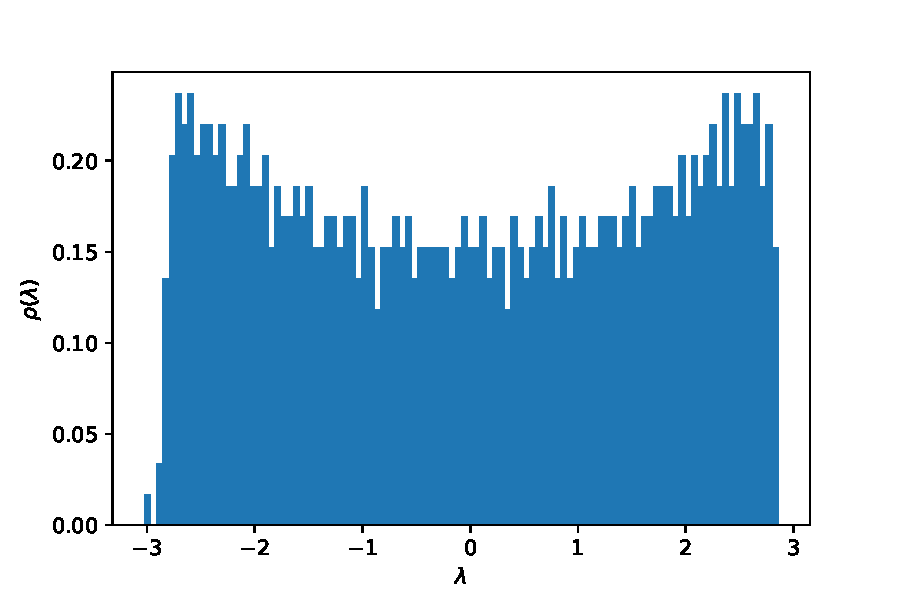
\includegraphics[width=0.8\textwidth]{../figures/ex3_spectrum_exact_diag.pdf}
    \caption{Spectral density of the Anderson Model for small disorder $W = \num{.3}$ on a large RRG of connectivity $c=3$ and $ N = 2^{10}$ nodes calculated by Direct Diagonalization of the Hamiltonian.}
    \label{fig:spectrum_exact_diagonalization}
\end{figure}

\begin{figure}[htpb]
    \centering
    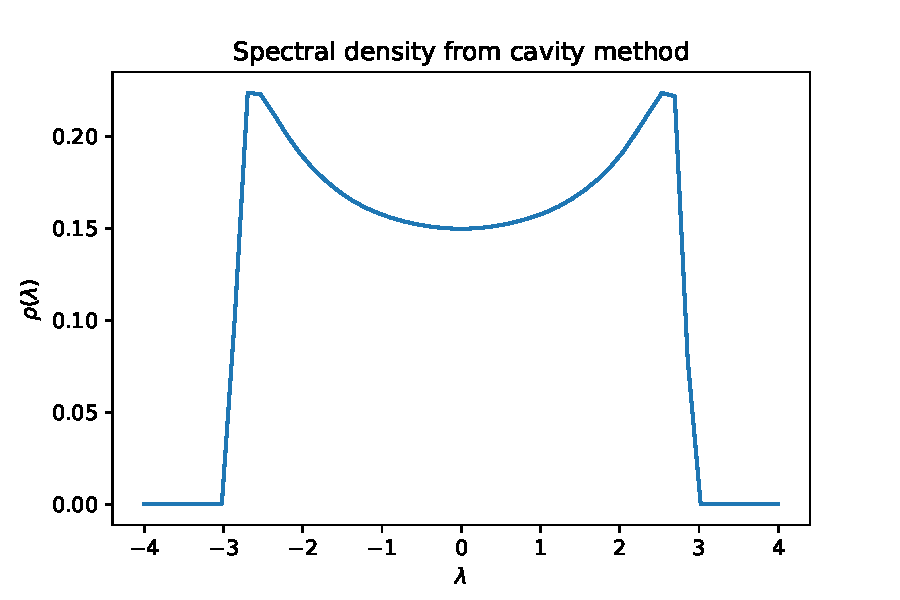
\includegraphics[width=0.8\textwidth]{../figures/ex3_spectrum_cavity.pdf}
    \caption{Spectral density of the Anderson Model for small disorder $W = \num{.3}$ on a large RRG of connectivity $c=3$ and $ N = 2^{10}$ nodes calculated by using the Cavity Method with $\varepsilon = \num{e-3}$ and the given cavity equations.}
    \label{fig:spectrum_cavity_method}
\end{figure}

To obtain a solid understanding of the Anderson Model's spectrum and to check them for consistency we use different techniques to calculate the spectral density.
Firstly we use the most straight-forward technique which is -- in this case -- Exact Diagonalization.
In Figure \ref{fig:spectrum_exact_diagonalization} you can see the eigenvalues of the system plotted in a histogram.
This gives us exactly the spectral density we are interested in.
\par

In similar fashion we have plotted the results of the cavity method in Figure \ref{fig:spectrum_cavity_method} such that we find the spectral density $\rho(\lambda)$ on the y-axis.
We can see that both results are consistent with each other.


\subsection{Spectrum from Population Method}

\begin{figure}[htpb]
    \centering
    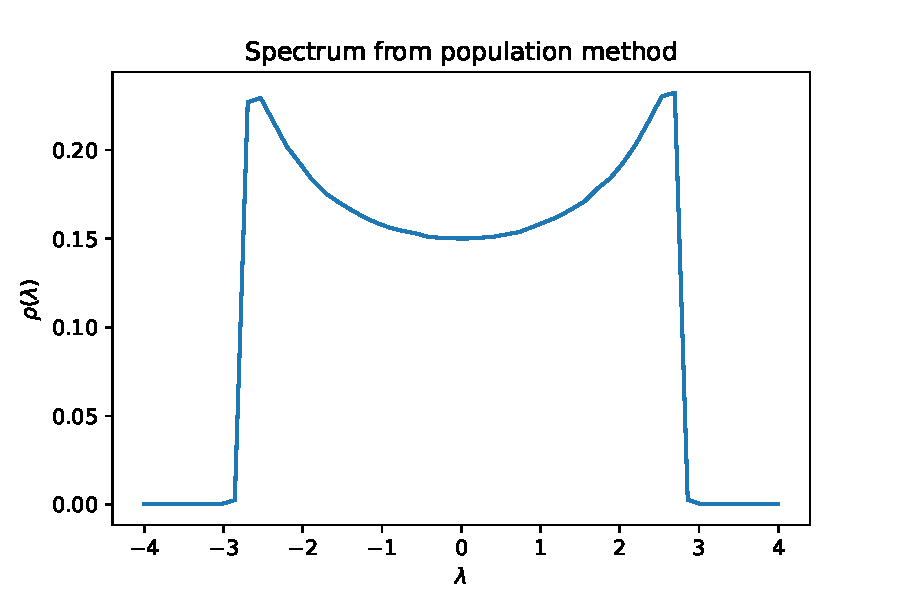
\includegraphics[width=0.8\textwidth]{../figures/ex3_spectrum_population.pdf}
    \caption{Spectral density of the Anderson Model for small disorder $W = \num{.3}$ on a large RRG of connectivity $c=3$ and $ N = 2^{10}$ nodes calculated by using the Population Method with $N_p = \num{e3}$ and the given cavity equations.}
    \label{fig:spectrum_population_method}
\end{figure}

We introduce another technique to analyze the system:
The Population Method uses a population of cavity precisions to calculate the marginal precisions of the system.
From Figure \ref{fig:spectrum_population_method} we can clearly see that this technique is also consistent with the other methods we have used to calculate the spectrum of the Anderson Hamiltonian.
\par

To ensure that the population of cavity precisions has reached equilibrium we use a stopping criterion.
Such we stop, when a whole sweep ($N_p$ updates) has not changed the absolute mean value of the cavity precisions by more than \num{e-4}.
We are aware that this criterion is not universal, but throughout experimenting with the algorithm we have seen that this is criterion works sufficiently well.


\subsection{Extended-Localized Transition}

To look at the transition from extended to Localized States we can analyze the typical value of the cavity variances $g = \nicefrac{i}{\omega}$



\ifSubfilesClassLoaded{
	% if it's compiled alone
}{
	% if it's compiled in the main file
    \newpage
}
\end{document}
